\todo{In this section I will discuss the information in the Figure~\ref{fig:previous_studies}}

% \citet{Lau+2020} find that the number of NSNS binaries in the Milky Way that would be detected by a 4 year LISA mission is 33, a factor of three times higher than our fiducial rate. This study incorporates \citet{Lau+2020} uses the same population synthesis code, COMPAS, as this study, though an earlier version. They make several different physical assumptions, using the \citet{Fryer+2012} \textit{rapid} remnant mass prescription, limiting the maximum neutron star mass to $2 \unit{M_{\odot}}$ and not implementing PISN. However, we note that none of these assumptions significantly affect the NSNS LISA detection rate (see bottom panel of Fig.\,\ref{fig:detection_rates}, models \modRapid{}, \modNSLow{} and \modNoPISN{}).

% We therefore surmise that the difference between our results is likely due to way in which we simulate the Milky Way. \citet{Lau+2020} assumes constant star formation, solar metallicity and distribute binaries following the blue light luminosity of the Milky Way, whilst we use the distributions from \citet{Frankel+2018} for the star formation rate, metallicity and positions. The \citet{Frankel+2018} star formation rate decreases over time and the metallicity distribution peaks above solar metallicity. Both of these changes could decrease the rate since most NSNS binaries in our sample have short inspiral times compared to the age of the Milky Way and higher metallicity would lead to increased stellar winds and hence less massive DCOs.

% \citet{Breivik+2020} find that LISA will detect 93 BHBH, 33 BHNS and 8 NSNS binaries in the Milky Way over a 4 year mission. Although these are significantly different from our fiducial results, we make many different physical assumptions, the most notable being that \citet{Breivik+2020} assumes the optimistic CE scenario. Thus it would be more prudent to compare to our results from model \modOpt{} in which we find 70, 38 and 15 detections respectively. The discrepancy in the NSNS rate is likely due to the fact that we assume that case BB mass transfer onto a NS is always stable but \citet{Breivik+2020} does not and this would significantly decrease our rate (see bottom panel of Fig.\,\ref{fig:detection_rates}, model \modCaseBB{}) . The remaining differences are likely due to using a different population synthesis code (COSMIC) and using a different model for the Milky Way, particularly the assumptions of two fixed metallicities.

\begin{figure*}[p]
    \centering
    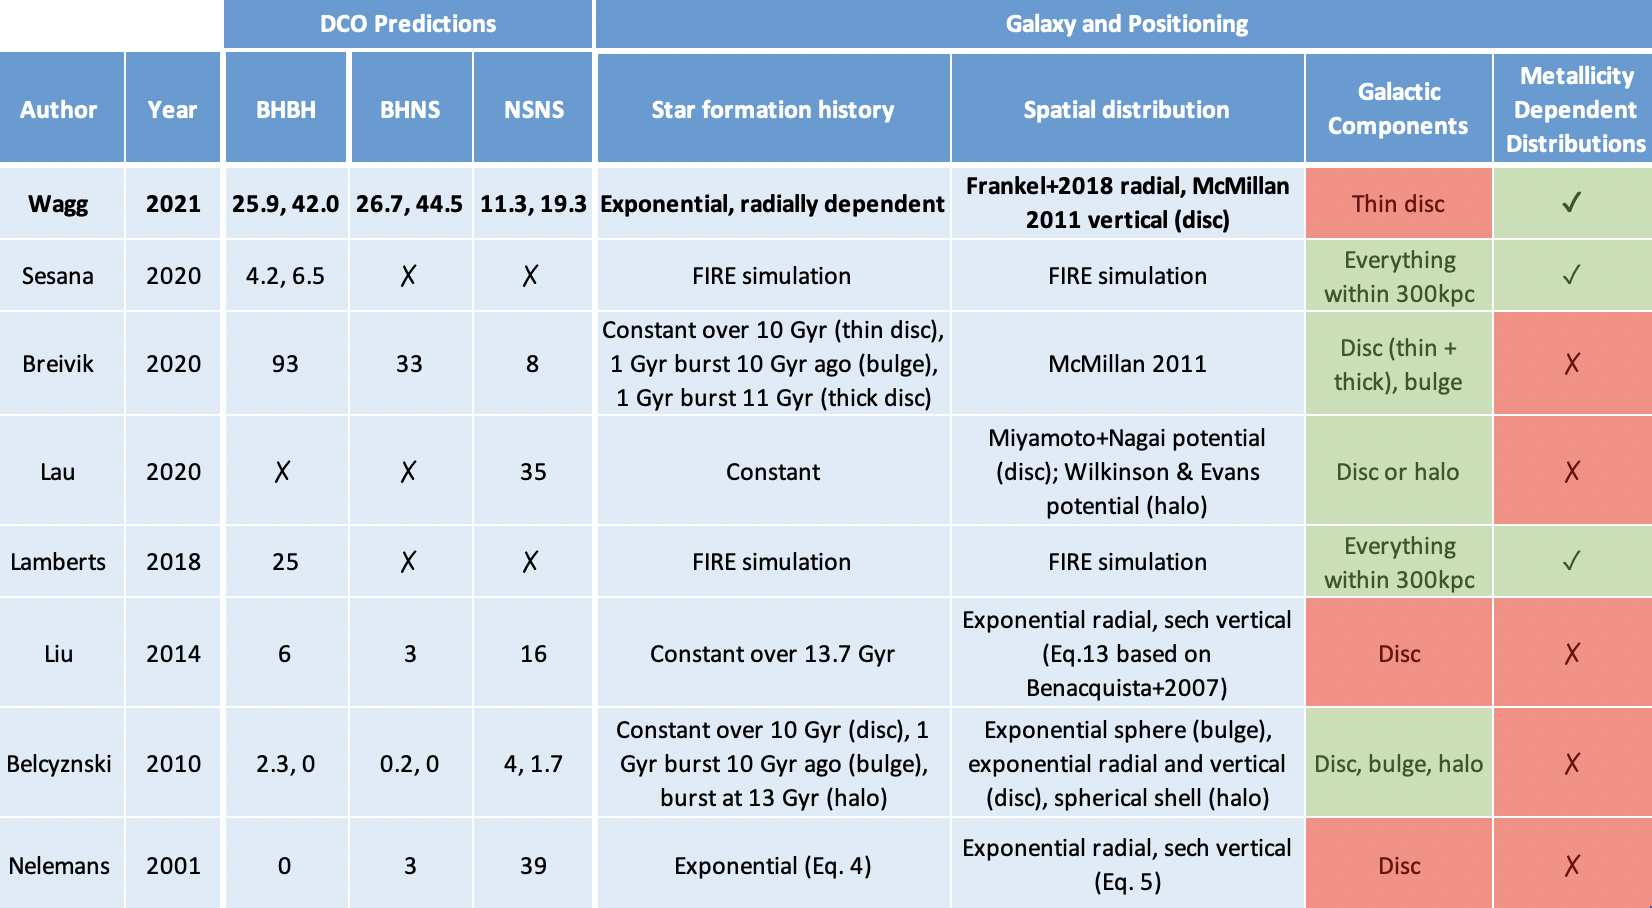
\includegraphics[width=\textwidth]{compare_dco_1.png}

    \vspace{0.5cm}

    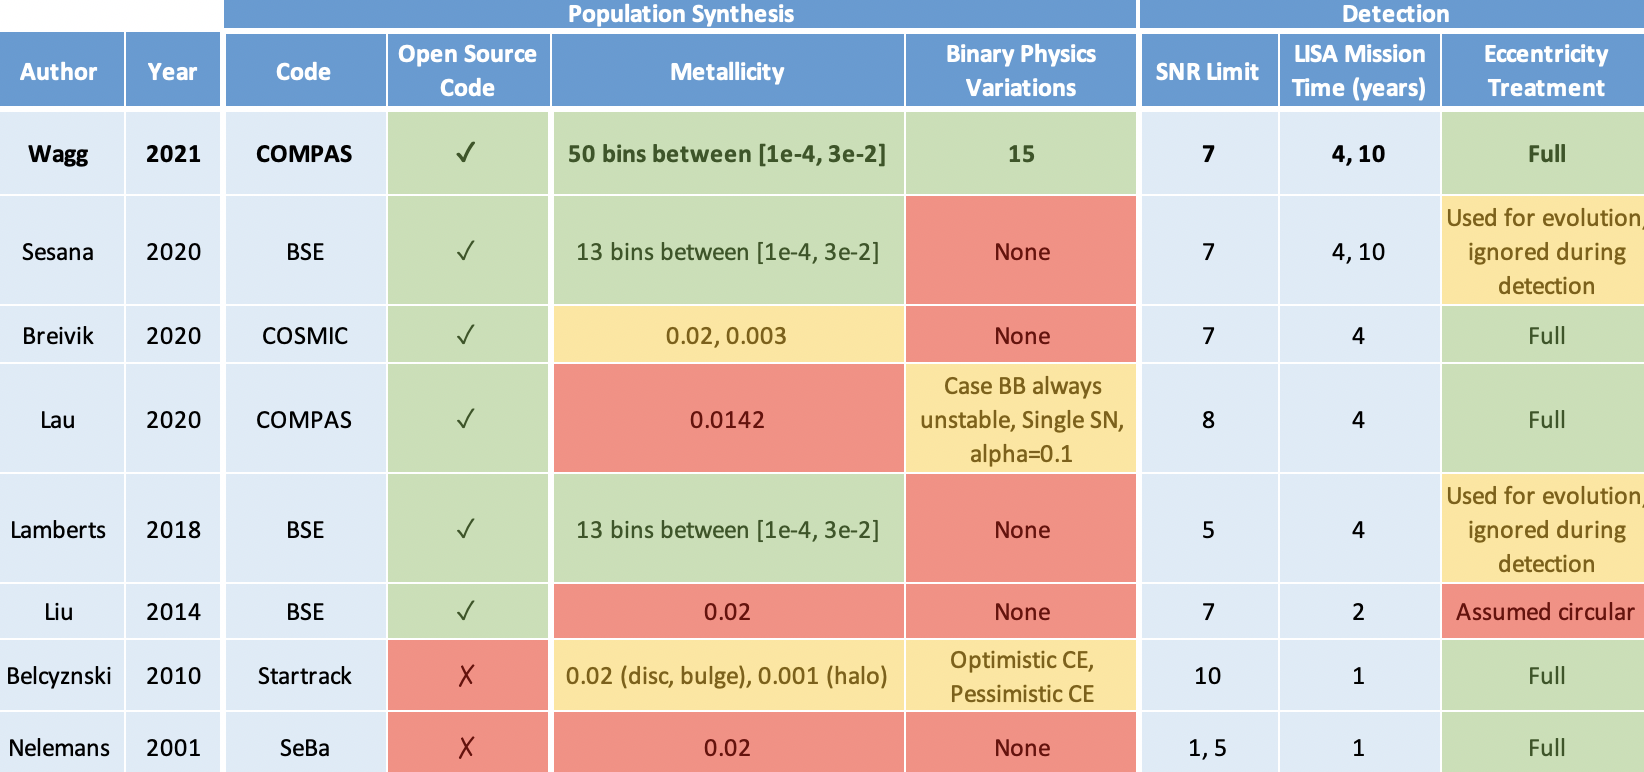
\includegraphics[width=\textwidth]{compare_dco_2.png}
    \caption{A table comparing previous studies of a similar nature to this work. The works listed in the table are \citet{Nelemans+2001,Belczynski+2010,Liu+2014,Lamberts+2018,Lau+2020,Breivik+2020,Sesana+2020}.}
    \label{fig:previous_studies}
\end{figure*}